\documentclass[,jou, draftfirst, a4paper,floatsintext]{apa6}
\usepackage{lmodern}
\usepackage{amssymb,amsmath}
\usepackage{ifxetex,ifluatex}
\usepackage{fixltx2e} % provides \textsubscript
\ifnum 0\ifxetex 1\fi\ifluatex 1\fi=0 % if pdftex
  \usepackage[T1]{fontenc}
  \usepackage[utf8]{inputenc}
\else % if luatex or xelatex
  \ifxetex
    \usepackage{mathspec}
  \else
    \usepackage{fontspec}
  \fi
  \defaultfontfeatures{Ligatures=TeX,Scale=MatchLowercase}
\fi
% use upquote if available, for straight quotes in verbatim environments
\IfFileExists{upquote.sty}{\usepackage{upquote}}{}
% use microtype if available
\IfFileExists{microtype.sty}{%
\usepackage{microtype}
\UseMicrotypeSet[protrusion]{basicmath} % disable protrusion for tt fonts
}{}
\usepackage{hyperref}
\hypersetup{unicode=true,
            pdftitle={Simulation-Based Power-Analysis for Factorial ANOVA Designs},
            pdfauthor={Daniël Lakens~\& Aaron Caldwell},
            pdfkeywords={power analysis, ANOVA, hypothesis test, sample size justification},
            pdfborder={0 0 0},
            breaklinks=true}
\urlstyle{same}  % don't use monospace font for urls
\usepackage{graphicx,grffile}
\makeatletter
\def\maxwidth{\ifdim\Gin@nat@width>\linewidth\linewidth\else\Gin@nat@width\fi}
\def\maxheight{\ifdim\Gin@nat@height>\textheight\textheight\else\Gin@nat@height\fi}
\makeatother
% Scale images if necessary, so that they will not overflow the page
% margins by default, and it is still possible to overwrite the defaults
% using explicit options in \includegraphics[width, height, ...]{}
\setkeys{Gin}{width=\maxwidth,height=\maxheight,keepaspectratio}
\IfFileExists{parskip.sty}{%
\usepackage{parskip}
}{% else
\setlength{\parindent}{0pt}
\setlength{\parskip}{6pt plus 2pt minus 1pt}
}
\setlength{\emergencystretch}{3em}  % prevent overfull lines
\providecommand{\tightlist}{%
  \setlength{\itemsep}{0pt}\setlength{\parskip}{0pt}}
\setcounter{secnumdepth}{0}
% Redefines (sub)paragraphs to behave more like sections
\ifx\paragraph\undefined\else
\let\oldparagraph\paragraph
\renewcommand{\paragraph}[1]{\oldparagraph{#1}\mbox{}}
\fi
\ifx\subparagraph\undefined\else
\let\oldsubparagraph\subparagraph
\renewcommand{\subparagraph}[1]{\oldsubparagraph{#1}\mbox{}}
\fi

%%% Use protect on footnotes to avoid problems with footnotes in titles
\let\rmarkdownfootnote\footnote%
\def\footnote{\protect\rmarkdownfootnote}


  \title{Simulation-Based Power-Analysis for Factorial ANOVA Designs}
    \author{Daniël Lakens\textsuperscript{1}~\& Aaron Caldwell\textsuperscript{2}}
    \date{}
  
\shorttitle{ANOVA Power}
\affiliation{
\vspace{0.5cm}
\textsuperscript{1} Eindhoven University of Technology, The Netherlands\\\textsuperscript{2} Department of Health, Human Performance and Recreation, University of Arkansas, USA}
\keywords{power analysis, ANOVA, hypothesis test, sample size justification\newline\indent Word count: Main text contains 5245 words.}
\usepackage{csquotes}
\usepackage{upgreek}
\captionsetup{font=singlespacing,justification=justified}

\usepackage{longtable}
\usepackage{lscape}
\usepackage{multirow}
\usepackage{tabularx}
\usepackage[flushleft]{threeparttable}
\usepackage{threeparttablex}

\newenvironment{lltable}{\begin{landscape}\begin{center}\begin{ThreePartTable}}{\end{ThreePartTable}\end{center}\end{landscape}}

\makeatletter
\newcommand\LastLTentrywidth{1em}
\newlength\longtablewidth
\setlength{\longtablewidth}{1in}
\newcommand{\getlongtablewidth}{\begingroup \ifcsname LT@\roman{LT@tables}\endcsname \global\longtablewidth=0pt \renewcommand{\LT@entry}[2]{\global\advance\longtablewidth by ##2\relax\gdef\LastLTentrywidth{##2}}\@nameuse{LT@\roman{LT@tables}} \fi \endgroup}


\usepackage{lineno}

\linenumbers

\authornote{All code used to create this manuscript is provided in an OSF repository at \url{https://osf.io/xxxxx/}.

Correspondence concerning this article should be addressed to Daniël Lakens, ATLAS 9.402, 5600 MB, Eindhoven, The Netherlands. E-mail: \href{mailto:D.Lakens@tue.nl}{\nolinkurl{D.Lakens@tue.nl}}}

\abstract{
To design informative studies where researchers plan to report results based on an analysis of variance (ANOVA), it is important to justify the sample size based on statistical power. Power analyses for factorial ANOVA designs are often challenging. First, current software solutions do not enable power analyses for more complex designs involving multiple within factors. Second, partial eta-squared or Cohen's f are required as input for the power analysis, but these effect sizes do not generalize to different experimental designs, and depend on the expected pattern of means. We have created R functions and an online Shiny app that performs simulations for ANOVA designs for up to three within or between factors, with an unlimited number of levels. Predicted effects are entered by specifying means, standard deviations, and correlations (for within factors). The simulation provides power calculations for all ANOVA main effects and interactions, and all independent comparisons between conditions. The simulation plots \emph{p}-value distributions for all tests, and allows researchers to select a range of options to correct for multiple comparisons. This tutorial will demonstrate how to perform power analysis for ANOVA designs. The simulations illustrate important factors that determine the statistical power of factorial ANOVA designs, and the code and Shiny app enable researchers without extensive programming experience to perform power analyses for a wide range of ANOVA designs. .


}

\begin{document}
\maketitle

When a researcher aims to test hypotheses based on an analysis of variance (ANOVA), the sample size of the study should be justified based on the statistical power of the test.
Statistical power is the probability of rejecting the null-hypothesis, given a specified effect size, alpha level, and sample size.
A study that has low power to detect effects the researcher is interested in leads to a high probability of saying there is no effect, when there actually is a true effect to be found.
Several excellent resources exist that explain power analyses, including books (Aberson, 2019; Cohen, 1988), general reviews (Maxwell, Kelley, \& Rausch, 2008), and practical primers (Brysbaert, 2019; Perugini, Gallucci, \& Costantini, 2018).
Whereas power analyses for simple comparisons are relatively easy to perform, power analysis for factorial ANOVA designs is a challenge.
Available software solutions do not provide easy options for more complex designs (e.g., a 2x2x2 design, where the first factor is manipulated between participants, and the last two factors are manipulated within participants).
The predicted effects often need to be specified as Cohen's f or partial eta squared (\(\eta_p^2\)), which are not the most intuitive way to specify a hypothesized pattern of results, and do not generalize to different experimental designs.
Simulations based on a specified pattern of means and standard deviations provides a more flexible approach to power analyses, but creating these simulations requires programming knowledge.
In this manuscript we provide R code and a Shiny app that can be used to perform power analyses for factorial ANOVA designs based on simulations, and calculate the statistical power based on a predicted pattern of means, standard deviations, and correlations (for within factors).
By simulating different factorial designs with a range of patterns of means, standard deiviations, and correlations, and calculating the effect sizes and statistical power for these designs, researchers can gain a better understanding of the factors that determine the statistical power of hypothesis tests.
After providing an introduction to statistical power in general, and for the \emph{F}-test specifically, we will demonstrate how the power of factorial ANOVA designs depends on the pattern of means across conditions, the number of factors and levels, and the sample size.
We also illustrate the importance of controlling the Type 1 error rate in exploratory ANOVA's to maintain the desired alpha level when performing multiple comparisons.

\hypertarget{calculating-power-in-anova-designs}{%
\section{Calculating Power in ANOVA Designs}\label{calculating-power-in-anova-designs}}

Imagine you plan to perform a study in which participants interact with an artificial voice assistant who sounds either cheerful or sad.
You measure how much 80 participants in each condition enjoy to interact with the voice assistant on a line marking scale (coded continuously from -5 to 5) and observe a mean of 0 in the sad condition, and a means of 1 in the cheerful condition, with an estimated standard deviation of 2.
After submitting your manuscript for publication, reviewers ask you to add a study with a neutral control condition to examine whether cheerful voices increase, or sad voices decrease enjoyment (or both).
Depending on what the mean in the neutral condition is, which sample size would you need to have a high powered study for the expected pattern or means?
A collaborator suggests to switch from a between design to a within design, to more efficiently collect the data.
Which consequence will switching from a between-participant to a within-participant design have on the required sample size?
Because the effect size in the first study could be considered \enquote{medium} based on the benchmarks by Cohen (1988), does it make sense to plan for a \enquote{medium} effect size in either the between or within ANOVA design?
And if you justify the sample size based on the power for the main effect for the ANOVA, will the study also have sufficient statistical power for the independent comparisons between conditions (or vice versa)?

\begin{figure}
\centering
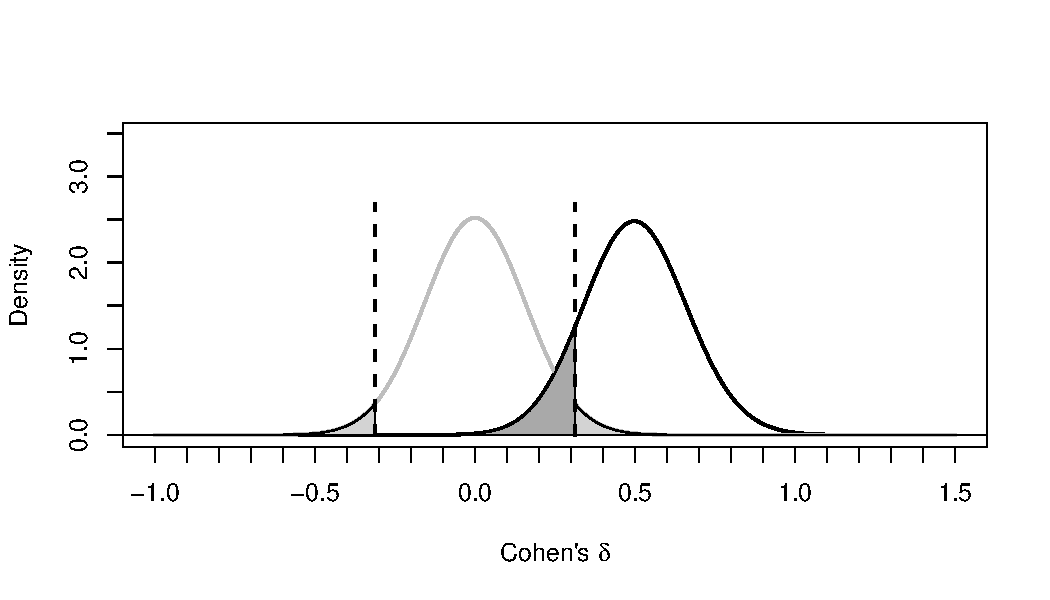
\includegraphics{0.1_Simulation_Based_Power_Analysis_For_Factorial_ANOVA_Designs_files/figure-latex/d-plot-1.pdf}
\caption{\label{fig:d-plot}Distribution of Cohen's d under the null-hypothesis (grey curve) and alternative hypothesis assuming d = 0.5 (black curve).}
\end{figure}

\begin{figure}
\centering
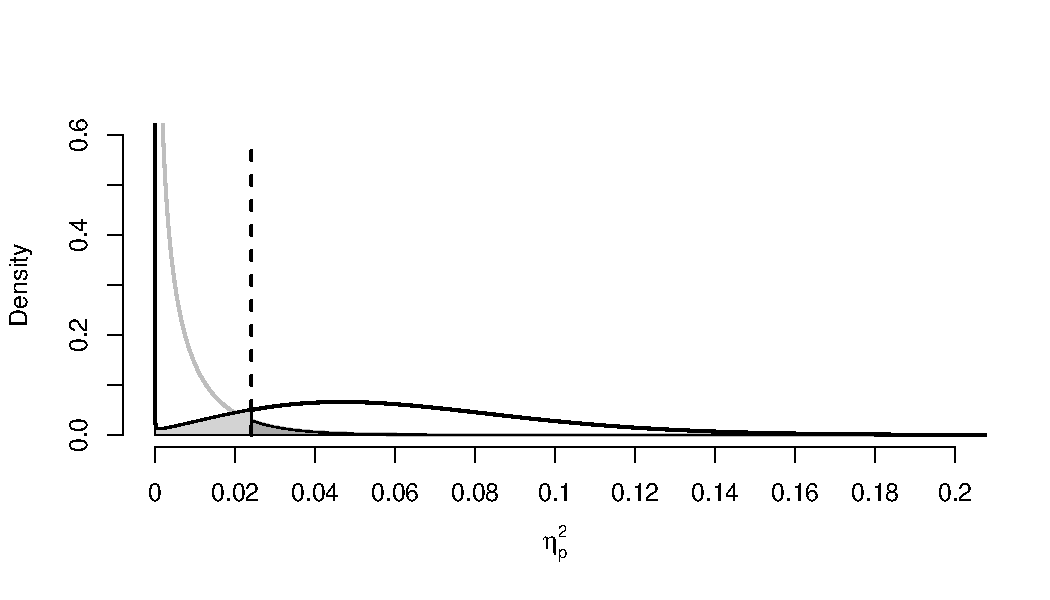
\includegraphics{0.1_Simulation_Based_Power_Analysis_For_Factorial_ANOVA_Designs_files/figure-latex/eta-plot-1.pdf}
\caption{\label{fig:eta-plot}Distribution of eta-squared under the null-hypothesis (grey curve) and alternative hypothesis assuming partial eta-squared = 0.0588 (black curve).}
\end{figure}

Let's consider the initial study described above, where enjoyment is measured when interacting with a cheerful or sad voice assistant.
We can test the difference between two means with a \emph{t}-test or a one-way ANOVA, and the two tests are mathematically equivalent.
Figure \ref{fig:d-plot} and Figure \ref{fig:eta-plot} visualize the distribution of the effect sizes Cohen's d (for the \emph{t}-test) and \(\eta_p^2\) (for the \emph{F}-test) that should be observed when there is no effect (grey curves) and when the observed difference between means equals the true effect (black curves)\footnote{For Shiny apps that allow you to dynamically change these figures, go to \url{http://shiny.ieis.tue.nl/d_p_power/} and \url{http://shiny.ieis.tue.nl/f_p_power/}}.
In both figures the light grey areas under the null-distribution mark the observed results that would lead to a Type 1 error (observing a statistically significant result if the null-hypothesis is true) and the dark grey areas under the curve marks the observed effect sizes that would lead to a Type 2 error.
A statistically significant result is observed whenever the observed effect size is larger than the critical value.
Critical values are often expressed as \emph{t}-values or \emph{F}-values, but for a given sample size can be expressed as effect sizes.
Given the sample size of 80 participants per group, effects are statistically significant when they are larger than d = 0.31 in a \emph{t}-test, or \(\eta_p^2\) = 0.02 for the \emph{F}-test.
The goal of a power analysis is to choose a sample size so that the probability of observing a statistically significant effect reaches a desired probability.
To calculate power, one has to specify the alternative hypothesis (the black curves in Figure \ref{fig:d-plot} and \ref{fig:eta-plot}).
If we assume the true effect size is d = 0.5 or \(\eta_p^2\) = 0.0588, and data from 80 participants in each condition is collected, in the long run 88.16\% of the observed effects will yield statistically significant results.

Two relationships between the \emph{t}-test and the \emph{F}-test when comparing two means are worth pointing out.
The \emph{t}-test examines the difference between means \$(m\_1 - m\_2), and the \emph{F}-test computes the ratio of the between group variance and the within group variance.
For two groups, the variance of the difference between two means is \((m_1 - m_2)^2\), and therefore \(F = t^2\).
The main difference between the \emph{t}-test and the \emph{F}-test is that the \emph{F}-test generalizes to more than two groups.
Second, for two groups the effect size for an ANOVA, Cohen's f, is half the size of the effect size for standardized mean differences, Cohen's d, or \(f = \frac{1}{2}d\).
Cohen's d is calculated by dividing the difference between means by the standard deviation, or
\begin{equation}
d = \frac{m_1-m_2}{\sigma}.
\end{equation}
If we have two groups with means of 1 and 2, and the standard deviation is 2, Cohen's d is (2-1)/2, or 0.5.
Cohen's f is the standard deviation of the population means divided by the population standard deviation (Cohen, 1988), or:
\begin{equation}
f = \frac{\sigma _{ m }}{\sigma}
\end{equation}
where for equal sample sizes,
\begin{equation}
\sigma _{ m } = \sqrt { \frac { \sum_ { i = 1 } ^ { k } ( m _ { i } - m ) ^ { 2 } } { k } }.
\end{equation}
Because Cohen's f is the effect size that is an essential factor when computing the power for factorial ANOVA designs, it is worth illustrating how it is calculated in an example.
If we again take two means of 1 and 2, and a standard deviation of 2, the grand mean is 1.5.
We subtract each condition mean from the grand mean, take the square, calculate the sum of squares, divide it by two, and take the square root.
\(\sigma_m = \sqrt{\frac{(1-1.5)^2+(2-1.5)^2}{2}} = \sqrt{\frac{0.25+0.25}{2}} = 0.5\), and \(f = \frac{0.5}{2} = 0.25.\)
We confirm that for a two group comparison, Cohen's f is half as large as Cohen's d.
Popular power analysis software such as G*Power (Faul, Erdfelder, Lang, \& Buchner, 2007) also allows researchers to enter the effect size for the power analsysi as partial eta-squared (\(\eta_p^2\)).
Partial eta-squared can be converted into Cohen's f:
\begin{equation}
f = \sqrt{\frac{\eta_p^2}{1-\eta_p^2}} \label{eq:eta-to-f}
\end{equation}
and Cohen's f can be converted into partial eta-squared:
\begin{equation}
\eta_p^2 = \sqrt{\frac{f^2}{f^2+1}} \label{eq:f-to-eta}
\end{equation}
In the example above, \(\eta_p^2 = 0.25^2/(0.25^2+1) = 0.0588\).
To calculate the statistical power assuming a specific true effect size we need the noncentrality parameter of the distribution.
In both Figure \ref{fig:d-plot} and Figure \ref{fig:eta-plot} we see examples of the non-central \emph{t}-distribution and non-central \emph{F}-distribution, or the shape of the expected test statistics when there is a true effect (the black curves).
Power calculations rely on the noncentrality parameter often referred to as lambda (\(\lambda\)). In a between-participants one-way ANOVA lambda is calculated as:
\begin{equation}
\lambda = f^2 \times N \label{eq:lambda}
\end{equation}
where f is Cohen's f and N is the total sample size.
Based on \(\lambda\) (which specifies the shape of the expected distribution under the specified alternative hypothesis) and the critical test statistic (which specifies the part of the distribution that is more extreme than the test statistic needed for a statistically significant test result) we can calculate how much of the distribution under the alternative hypothesis will be statistically significant in the long run (i.e., the area under the black curve in Figure \ref{fig:d-plot} and \ref{fig:eta-plot} to the right of the critical effect size).

\hypertarget{simulating-statistical-power-for-different-factorial-designs}{%
\section{Simulating Statistical Power for Different Factorial Designs}\label{simulating-statistical-power-for-different-factorial-designs}}

We have created R code and a Shiny app that simulate factorial ANOVA designs.
At the core, the code generates data for each condition in the design, performs an ANOVA.
The simulation also performs \emph{t}-tests for all independent comparisons between conditions.
Then the percentage of significant results (i.e., the power) is calculated (after correcting the alpha level for multiple comparisons if desired) and average effect size estimates are computed for all tests.
The software requires specifying the design of the study, by providing the number of levels for each factor, and indicating whether the factor is measured between or within participants. Our initial study above is a \enquote{2b} or two level between-participant design.
For ease of interpretation the factors and levels can be named (for our example, Condtion, cheerful, sad).
The planned sample size should be specified, which is 80 participants in each between-participant condition.
The means for each condition should be specified (0 and 1), as well as the standard deviation (2).
For within designs the correlation between variables should be specified.
When these variables are provided, the design is set up for the simulation.
For a visual confirmation of the input, a figure is created that displays the means (see Figure \ref{fig:mean-plot2}).

\begin{figure}
\centering
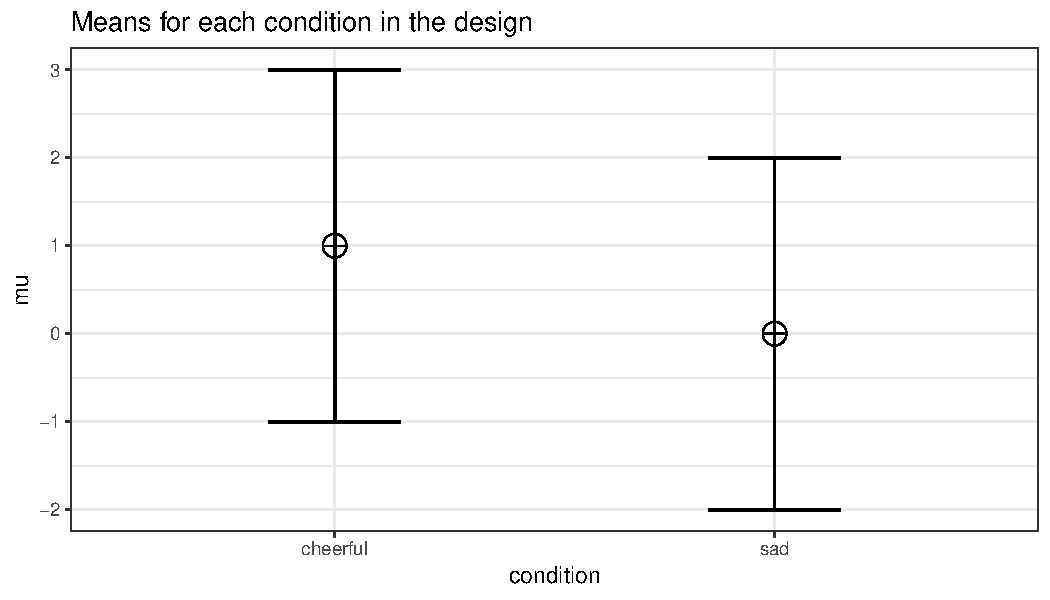
\includegraphics{0.1_Simulation_Based_Power_Analysis_For_Factorial_ANOVA_Designs_files/figure-latex/mean-plot2-1.pdf}
\caption{\label{fig:mean-plot2}Vizualization for the expected means and confidence intervals for the two conditions.}
\end{figure}

The results of a simulation study will vary each time the simulation is performed (but can be made reproducible by specifying a \enquote{seed} number).
Results become more stable, the more simulations are performed, but the simulations also take longer.
To perform the simulations, you specify the number of simulations, the alpha level for the tests, and any adjustment for multiple comparisons for the ANOVA.
If 100.000 simulations are performed in R with a seed set to 2019 (these settings will be used for all simulation results in this manuscript), we see the statistical power (based on the percentage of \emph{p} \textless{} \(\alpha\) results) is 95 and the average effect size is 0.07.
The simulation also provides the results for the independent comparisons, based on \emph{t}-tests comparing each condition.
Since there are only two groups in this example, the results for the statistical power of the independent comparison is identical, but the effect size is -0.54, which is the effect size in Cohen's d.~

Now the basic idea behind the simulation is clear, we can start exploring how changing the experimental design influences our power, and answer some of the questions our hypothetical researcher was confronted with when designing a follow-up study.
We will first examine what happens if we add a third condition to the design.
Let's assume we expect the neutral voice condition to fall either between the cheerful and sad conditions, or perhaps to be equal to the cheerful condition (based on the idea that the sad voice leads to less enjoyment, but the cheerful voice does not lead to more enjoyment).
The design now has 3 between-participant conditions, and we can explore what happens if we would collect 80 participants in each condition.

If we assume the mean falls exactly between between the cheerful and sad conditions the simulations show the statistical power for our design is reduced to 82\%, and the effect size is 0.05.
If we assume the mean the mean is equal to the cheerful condition, the power increases to 92\%.
Compared to the two group design, three things have changed.
First, an additional group was added to the design.
This increases the numerator degrees of freedom, and makes the non-central \emph{F}-distribution more similar to the central \emph{F}-distribution, and reduces the statistical power.
Second, the total sample size is 50\% larger than in the initial two-group study, which increases the statistical power.
Third, the effect size has decreased, which reduces the statistical power.
The exact effect of these three changes on the statistical power is difficult to predict.
The most important conclusion based on these simulations is that changing an experimental design can have several opposing effects on the power of a study, depending of the pattern of means.
One can not assume the effect size remains unchanged, when the design changes.

What happens if we would perform the second study as a within-participants design?
Instead of collecting three groups of participants, we only collect one group, and let this group evaluate the cheerful, neutral, and sad voice assistants.
The sample size needed in a within-design (\(N_W\)), relative to the sample needed in between-design (\(N_B\)), is (from Maxwell \& Delaney, 2004, p.~562, formula 47):
\begin{equation}
N_{W}=\frac{N_{B}(1-\rho)}{a} \label{eq:within-n}
\end{equation}
Here \emph{a} is the number of within-participant levels, \(\rho\) is the correlation between the measurements, and the formula assumes normal distributions and compound symmetry, and ignores the difference in degrees of freedom between the two types of tests, so it is a rough (but useful) approximation.
Whenever the correlation between dependent measures is positive, the sample size that is needed in a within-participants condition will be smaller than the requires sample size for a between-participants condition.

We need to predict what the correlation between the dependent variables will be, ideally based on data from previous experiments.
If we plan to collect 80 participants, and assume the correlation between all dependent variables is 0.5, the power for the repeated-measures ANOVA is 97\%.
Note that simulation studies allow for great flexibility, and the Shiny app and ANOVApower package allow researchers to enter a correlation matrix that specifies the expected correlations between each individual pair of measurements, instead of assuming the correlations between all dependent variables are identical.

\hypertarget{power-for-interactions}{%
\section{Power for Interactions}\label{power-for-interactions}}

The effect size for an ANOVA design depends on the pattern of means.
Let's assume the researcher plans to perform a follow-up experiment where in addition to making the voice sound cheerful or sad, a second factor is introduced by making the voice sound more robotic compared to the default human-like voice.
Different patterns of results could be expected.
Either the same effect is observed for robotic voices, or no effect is observed for robotic voices, or the opposite effect is observed for robotic voices (a \enquote{Marvin-the-Depressed-Robot Effect}).
In the first case, we will only observe a main effect of voice, but in the other two scenarios there is an interaction effect between human-likeness of the voice and the emotional tone of the voice. We can start by simulating the power for a cross-over interaction for a 2x2 between-participant design with 80 participants in each group (see Figure \ref{fig:mean-plot} for the expected pattern of means).

\begin{figure}
\centering
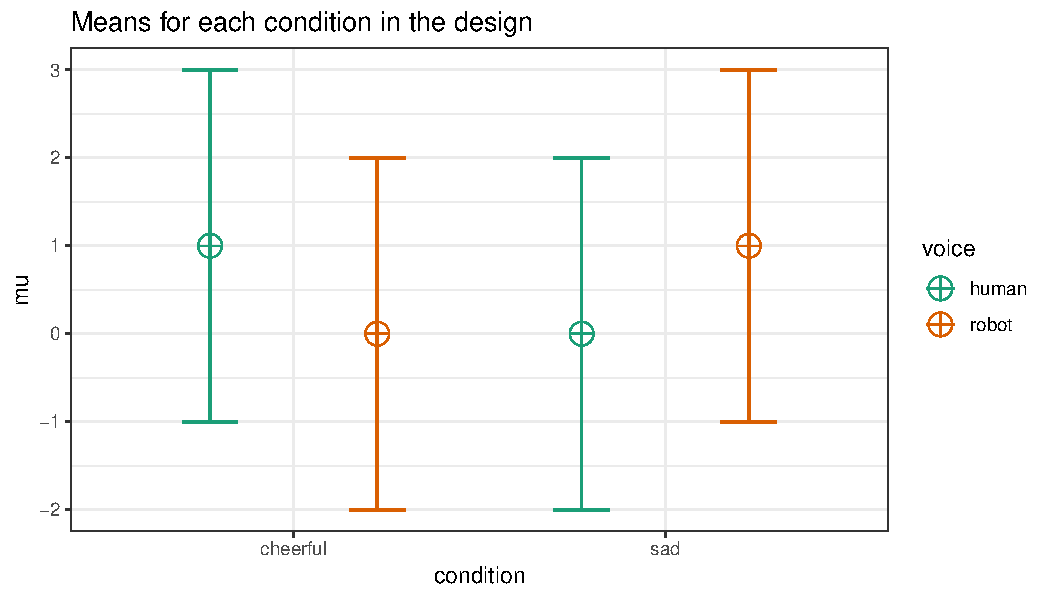
\includegraphics{0.1_Simulation_Based_Power_Analysis_For_Factorial_ANOVA_Designs_files/figure-latex/mean-plot-1.pdf}
\caption{\label{fig:mean-plot}Vizualization for the expected means and confidence intervals for a crossover interaction.}
\end{figure}

Mathematically the interaction effect is computed as the cell mean minus the sum of the grand mean, the marginal mean in row i minus the grand mean, and the marginal mean in column j minus grand mean. For example, for the cheerful human-like voice condition this is 1 (the value in the cell) - (0.5 {[}the grand mean{]} + 0.5 {[}the cell mean minus the marginal mean in row 1, 0.5{]} + 0.5 {[}the cell mean minus the marginal mean in column 2, 0.5{]}). 1 - (0.5 + (0.5) + (0.5)) = -0.5.
Completing this for all four cells gives the values -0.5, 0.5, 0.5, -0.5.
Cohen's f is then \(f = \frac { \sqrt { \frac { -0.5^2 + 0.5^2 + 0.5 + -0.5^2 } { 4 } }}{ 2 } = 0.25\).
Cohen's f for the 2x2 design is the same as for the two-group design, but we have collected twice as many observations (4 times 80 participants).
Simulations show we have would have exactly the same power for a cross-over (also called \enquote{disordinal}) interaction if we halved the sample size per group from 80 to 40.
Main effects in an ANOVA are based on the means for one factor averaged over the other factors (e.g., the main effect of human-like versus robot-like voice, irrespective of whether it is cheerful or sad).
The interaction effect, which can be contrast coded as 1, -1, -1, 1, is similarly a test of whether the effects are non-additive based on the scores in each cell, where the null-hypothesis of no additive effect can be rejected if the deviation expected when effects in each cell would be purely additive can be rejected.
The key insight here is that the total sample size determines the power (cf.~Westfall, 2015).

We can also examine what the statistical power would be if the pattern of results indicated that there was no difference in interacting with a cheerful of sad conversational agent with a robot voice.
In this case, we expect an \enquote{ordinal} interaction (the means for the human-like voice are never lower than the means for the robot-like voice, and thus there is no cross-over effect).
The pattern of means is now 1, 0, 0, 0, with only a single mean that differs from the rest.
As has been pointed out (Giner-Sorolla, 2018; Simonsohn, 2014) these designs require larger samples to have the same power to detect the interaction compared to the two-group comparison.
The reason for this is that the effect size is only half as large, with Cohen's f = 0.125 (compared to 0.25 in the cross-over interaction).
To achieve the same power as for the two-group comparison, a total sample size of 635 is required, almost four times as large as the sample size for the two-group comparison.

The power in the 2x2 ordinal interaction where only one cell mean differs from the other three cell means is identical to the power we would have if the single mean was twice as far from the remaining means (for a pattern of means of 2, 0, 0, 0).
Similarly, if we would examine a 2x2x2 interaction where only one cell differs from the other means, Cohen's f would be 0.25 only when the pattern of means is 4, 0, 0, 0, 0, 0, 0, 0 across the eight cells. The take-home message is that the effect size, and thus the power, for interactions in ANOVA designs depends on the pattern of the means.
A \enquote{medium} effect size translates into a much more extreme pattern of means in an ordinal interaction than in a disordinal (crossover) interaction, or in a 2x2x2 interaction compared to a 2x2 interaction.
For this reason, it is not very intuitive to start a power analysis based on an assumption of the effect size.
The same effect size can represent very different patterns of means depending on the type of interaction and the number of factors (see also Perugini et al. (2018)).
Instead, it might be more intuitive to think about the pattern of means that you expect, and compute the corresponding Cohen's f.~

\hypertarget{power-for-within-designs}{%
\section{Power for Within Designs}\label{power-for-within-designs}}

Whereas in an independent \emph{t}-test the two measurements are uncorrelated, in a within design the observations are correlated.
This has an effect on the standard deviation of the difference scores.
In turn, because the standardized effect size is the mean difference divided by the standard deviation of the difference scores, the correlation has an effect on the standardized mean difference in a within design, referred to as Cohen's \(d_z\) (because it is the effect size of the difference score between x and y, z). The relation is:
\begin{equation}
\sigma_{z}=\sigma\sqrt{2(1-\rho)}
\end{equation}
Therefore, the relation between \(d_z\) and d is \(\sqrt{2(1-\rho)}\).
As Cohen (1988) writes: \enquote{In other words, a given difference between population means for matched (dependent) samples is standardized by a value which is \(\sqrt{2(1-\rho)}\) as large as would be the case were they independent}.
If we enter a correlation of 0.5 in the formula, we get \(\sqrt{2(0.5)}=1\).
In other words, when the correlation is 0.5, d = \(d_z\). When there is a strong correlation between dependent variables, for example \emph{r} = 0.9, we get \(d=d_{z}\sqrt{2(1-0.9)}\), and a \(d_z\) of 1 in a within design is equivalent to a d = 0.45 in a between design.
Reversely, \(d_{z}=\frac{d}{\sqrt{2(1-r)}}\), so with a \emph{r} = 0.9, a d of 1 would be a \(d_z\) = 2.24.
Some consider this increase in \(d_z\) compared to d when observations are strongly correlated an \enquote{inflation} when effect sizes are estimated, but since the reduction in the standard deviation of the difference scores due to the correlation makes it easier to distinguish signal from noise in a hypothesis test, Cohen's \(d_z\) is the effect size used in power analyses.

There is no equivalent Cohen's \(f_z\) for a within-participant ANOVA, as there is a Cohen's \(d_z\) for a dependent \emph{t}-test. Instead, the value for lambda (\(\lambda\)) is adjusted based on the correlation. For a one-way within-participant design lambda is calculated as in Equation \eqref{eq:lambda}, multiplied by \emph{u}, a correction for within-designs, calculated as:
\begin{equation}
u = \frac{k}{1-\rho}
\end{equation}
where k is the number of levels of the within-participant factor, and \(\rho\) is the correlation between dependent variables.
If the correlation is 0, Equation \eqref{eq:within-n} shows that the required sample size is reduced only because each participants contributes multiple measurements, so for two groups the required sample size is halved.
If the correlation is larger than zero, both for the dependent \emph{t}-test as for the repeated measures ANOVA, the required sample size to achieve a desired level of statistical power decreases as the correlation increases.
Note that in the simulation, the correlation can be specified for each pair of measurements, but in the formula the correlation is assumed to be the same for all pairs.

Cohen's f is identical in within and between designs.
However, Equation \eqref{eq:eta-to-f} and \eqref{eq:f-to-eta} no longer hold when measurements are correlated.
The average effect size for a between design with 80 participants in each condition, means of 1, 0.5, and 0, and a standard deviation of 2 was 0.05, while the estimated effect size increased to 0.12 with a correlation of 0.7 between dependent measurements.
The default settings in G*Power expect an f or \(\eta_p^2\) that does not incorporate the correlation, while the correlation is incorporated in the output of software package such as SPSS.
For a one-way within design, Cohen's f can be converted into Cohen's f as SPSS provides it through:
\begin{equation}
f^2_{SPSS} = f^2 \times \frac{k}{k-1} \times \frac{n}{n-1} \times \frac{1}{1-\rho}
\end{equation}
and subsequently tranformed to \(\eta_p^2\) through Equation \eqref{eq:f-to-eta}.

\hypertarget{power-for-simple-comparisons}{%
\section{Power for Simple Comparisons}\label{power-for-simple-comparisons}}

Although an initial goal when performing an ANOVA might be to test the \emph{omnibus null hypothesis}, which answers the question whether there are \emph{any} differences between group means, we often want to know which groups differ from each other. Thus, an ANOVA is often followd up by individual comparisons (whether \emph{planned} or \emph{post-hoc}).
One feature of the simulation is that it provides the statistical power for all individual comparisons that can be performed.
The power and effect size estimates are based on \emph{t}-test.
Although \emph{t}-t-tests ignore the variance estimates from other groups (when factors have more than 2 levels), which can yield power benefits, the homogeneity assumption is often not warranted in psychological research.
Violations of the homogeneity assumption impact Type 1 error rates (Delacre, Lakens, Mora, \& Leys, 2018).\\
Furthermore, \emph{t}-tests allow researchers to specify directional predictions which increase the power of individual comparisons.

Power analysis for individual comparisons are relatively straightforward and can easily be done in all power analysis software.
Nevertheless, in our anecdotal experience evaluating sample size justifications for an ethical review board researchers often forget to power their ANOVA designs for follow-up tests.
We hope that providing a complete overview of the tests a researcher might be interested in will prevent this.
Furthermore, researchers need to take the correlation between dependent measures into account (e.g., enter Cohen's \(d_z\) instead of d), which the simulation does automatically.

Although the power for the cross-over interaction is high (97\%), the power for the independent between-participant comparisons where there is a difference is only 33\%, while the power for correlated between-participant effects is 69\%.
Sometimes the interaction in the ANOVA will have more power than the independent comparisons (i.e., in the case of a cross-over interaction) and sometimes the power for the interaction will be lower than the poewr for independent comparisons.
It is always important to check if you have adequate power for all tests you plan to perform.

\hypertarget{type-1-error-control-in-exploratory-anovas}{%
\section{Type 1 Error Control in Exploratory ANOVA's}\label{type-1-error-control-in-exploratory-anovas}}

In a 2x2x2 design, an ANOVA will give the test results for three main effects, three two-way interactions, and one three-way interaction.
Because seven statistical tests are performed, the probability of making at least one Type 1 error in a single exploratory 2x2x2 ANOVA is \(1-(0.95)^7\) = 30\%.
It is therefore important to control error rates when performing multiple comparisons (Cramer et al., 2014).
Several techniques to control error rates exist, of which the best known is the Bonferroni adjustment.
The Holm procedure is slightly more powerful than the Bonferroni adjustment, without requiring additional assumptions (for other approaches, see Bretz, Hothorn, \& Westfall, 2011).
By specifying the adjustment for multiple comparisons in the simulation it is possible to make sure that you will not conclude there is an effect in any of the tests more often than a desired overall Type 1 error rate.
Because the adjustment for multiple comparisons lowers the alpha level, it also lowers the statistical power.
When designing a study where you will perform multiple comparisons, it is important to take into account the corrected alpha level when determining the required sample size, both for the ANOVA tests, as for the independent comparisons.

If we revisited the 2x2 mixed ANOVA discussed in the section on independent comparison, and apply a Holm correction for multiple comparisons, we see power for the interaction is reduced from 97\% without applying a correction, to 92\% after correcting for multiple comparisons.
There are three tests for a 2x2 design (two main effects, one interaction), but 6 independent comparisons between the four conditions, and thus the correction for multiple comparisons has a stronger effect on the independent comparisons.
For example, the power for the dependent \emph{t}-test comparing two within-participant conditions falls from 69\% without correcting for multiple comparisons, to 47\% when adjusting the alpha level for the 6 possible comparisons between the four conditions.
These simulations should reveal the cost of exploring across all possible comparisons while controlling error rates.
It is often advisable to preregister specific tests that are of interest to a researchers.
If one is really interested in all possible comparisons, but wants to control the probability of incorrectly assuming there is an effect, the reduction in power due to the lower alpha level should be counteracted by increasing the sample size to maintain an adequate level of power for both the ANOVA as the independent comparisons.

\hypertarget{p-value-distributions}{%
\section{P-value distributions}\label{p-value-distributions}}

Statistical power is the probability of, in the long run, observing a \emph{p}-value smaller than the alpha level.
One intuitive way to illustrate this concept is to plot the distribution of \emph{p}-values for all simulations.
The simulation code automatically stores plots for \emph{p}-value distributions for each simulation, both for the ANOVA results, as for the independent comparisons.
In Figure \ref{fig:p-plot} we see that from 100 simulations that are performed, more fall below the alpha level for the tests in the top and bottom \emph{p}-value distributions, indicating greater statistical power.
For the two tests in the middle \emph{p}-value distributions, we see that \emph{p}-value are uniformly distributed because there is no true effect, and thus we only see Type 1 errors.

\begin{figure}
\centering
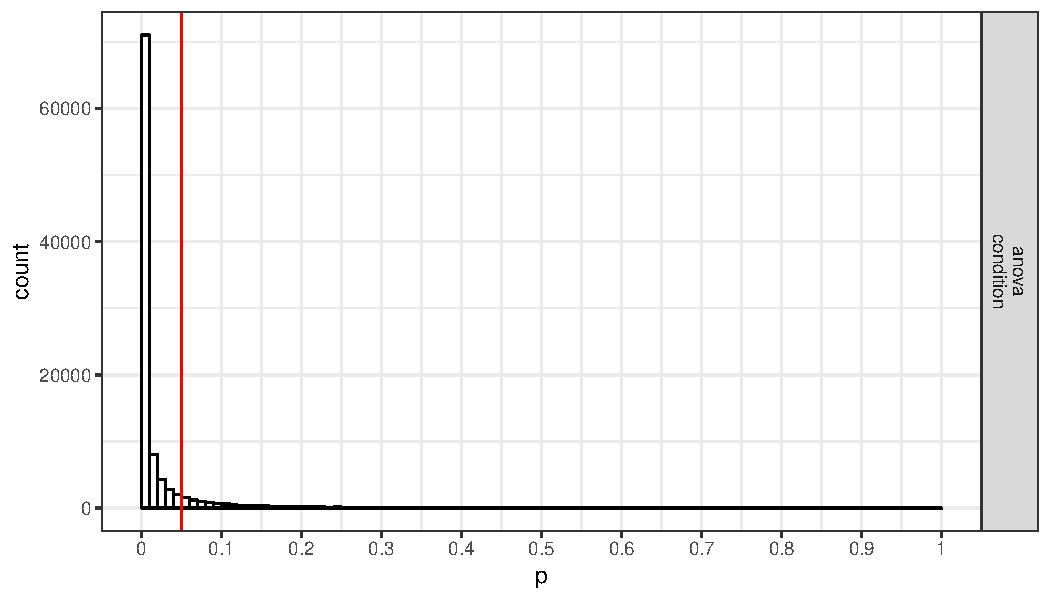
\includegraphics{0.1_Simulation_Based_Power_Analysis_For_Factorial_ANOVA_Designs_files/figure-latex/p-plot-1.pdf}
\caption{\label{fig:p-plot}Distribution of p-values for 6 independent comparisons between four conditions of a 2x2 mixed ANOVA}
\end{figure}

\hypertarget{conclusion}{%
\section{Conclusion}\label{conclusion}}

When designing informative studies, it is important to carefully justify the sample size.
Determining the sample size that is required for a well-powered factorial ANOVA design with multiple factors is quite complex, and existing power analysis software lacks options to calculate power for designs with multiple within-participant factors.
Simulation based approaches can help to provide insights into the factors that determine the statistical power in factorial ANOVA designs.
If researchers are able to specify the expected pattern of means, standard deviations, and correlations between variables, they can use simulations to examine the required sample size for factorial designs that consists of multiple factors and include both within as between participant factors.
The R package and Shiny app that accompany this paper enable researchers to perform simulations for factorial experiments of up to three factors and any number of levels, making it easy to perform simulation-based power analysis without extensive programming experience.

\newpage

\hypertarget{references}{%
\section{References}\label{references}}

\setlength{\parindent}{-0.5in}
\setlength{\leftskip}{0.5in}

\hypertarget{refs}{}
\leavevmode\hypertarget{ref-aberson_applied_2019}{}%
Aberson, C. L. (2019). \emph{Applied Power Analysis for the Behavioral Sciences: 2nd Edition} (2 edition.). New York: Routledge.

\leavevmode\hypertarget{ref-bretz_multiple_2011}{}%
Bretz, F., Hothorn, T., \& Westfall, P. H. (2011). \emph{Multiple comparisons using R}. Boca Raton, FL: CRC Press.

\leavevmode\hypertarget{ref-brysbaert_how_2019}{}%
Brysbaert, M. (2019). How many participants do we have to include in properly powered experiments? A tutorial of power analysis with some simple guidelines. \emph{Journal of Cognition}.

\leavevmode\hypertarget{ref-cohen_statistical_1988}{}%
Cohen, J. (1988). \emph{Statistical power analysis for the behavioral sciences} (2nd ed.). Hillsdale, N.J: L. Erlbaum Associates.

\leavevmode\hypertarget{ref-cramer_hidden_2014}{}%
Cramer, A. O., van Ravenzwaaij, D., Matzke, D., Steingroever, H., Wetzels, R., Grasman, R. P., \ldots{} Wagenmakers, E.-J. (2014). Hidden multiplicity in multiway ANOVA: Prevalence, consequences, and remedies. \emph{arXiv Preprint arXiv:1412.3416}.

\leavevmode\hypertarget{ref-delacre_why_2018}{}%
Delacre, M., Lakens, D., Mora, Y., \& Leys, C. (2018). Why Psychologists Should Always Report the W-test Instead of the F-Test ANOVA. \emph{PsyArXiv}. doi:\href{https://doi.org/10.17605/OSF.IO/WNEZG}{10.17605/OSF.IO/WNEZG}

\leavevmode\hypertarget{ref-faul_gpower_2007}{}%
Faul, F., Erdfelder, E., Lang, A.-G., \& Buchner, A. (2007). GPower 3: A flexible statistical power analysis program for the social, behavioral, and biomedical sciences. \emph{Behavior Research Methods}, \emph{39}(2), 175--191. doi:\href{https://doi.org/10.3758/BF03193146}{10.3758/BF03193146}

\leavevmode\hypertarget{ref-giner-sorolla_powering_2018}{}%
Giner-Sorolla, R. (2018, January). Powering Your Interaction. \emph{Approaching Significance}.

\leavevmode\hypertarget{ref-maxwell_sample_2008}{}%
Maxwell, S. E., Kelley, K., \& Rausch, J. R. (2008). Sample Size Planning for Statistical Power and Accuracy in Parameter Estimation. \emph{Annual Review of Psychology}, \emph{59}(1), 537--563. doi:\href{https://doi.org/10.1146/annurev.psych.59.103006.093735}{10.1146/annurev.psych.59.103006.093735}

\leavevmode\hypertarget{ref-perugini_practical_2018}{}%
Perugini, M., Gallucci, M., \& Costantini, G. (2018). A Practical Primer To Power Analysis for Simple Experimental Designs. \emph{International Review of Social Psychology}, \emph{31}(1), 20. doi:\href{https://doi.org/10.5334/irsp.181}{10.5334/irsp.181}

\leavevmode\hypertarget{ref-simonsohn_no-way_2014}{}%
Simonsohn, U. (2014, March). No-way Interactions. \emph{Data Colada}.

\leavevmode\hypertarget{ref-westfall_think_2015}{}%
Westfall, J. (2015, May). Think about total N, not n per cell. \emph{Cookie Scientist}.


\end{document}
